%%%%%%%%%%%%%%%%%%%%%%%%%%%%%%%%%%%%%%%%%%%%%%%
%
%   Families of Traffic Forecasting Problems
%
%%%%%%%%%%%%%%%%%%%%%%%%%%%%%%%%%%%%%%%%%%%%%%%

%\usepackage{cite}
%\usepackage{multirow}
%\usepackage{rotating} 
%\usepackage[table,xcdraw]{xcolor}
%\usepackage{float}
%\usepackage[utf8]{inputenc}
%\usepackage{amsmath,amssymb,amsfonts}
%\usepackage{algorithmic}
%\usepackage{graphicx}
%\usepackage{textcomp}
%\usepackage{rotating}
%\usepackage{verbatim}


\section{Experimental Results}
\label{sec:4_5_Expsetup}

In this section, the proposed HTL, CORAL \cite{sun2016return}, and CDTL \cite{yang2021concept}, and Melanie \cite{dong2019multistream} algorithms are compared. Three subsections are introduced: the first section focuses on the experimental setup; second, a discussion on data streams to apply our experiments on heterogeneous and homogeneous source domains, including a comparison to evaluate the runtime factor between all methods; and finally, a comparison is made between online learning and chunk-based concept drift.


\subsection{Experimental setup}
The evaluation of Heterogeneous Taxonomy Learning (HTL) involves a comparison with CORAL \cite{sun2016return}, CDTL \cite{yang2021concept}, and Melanie \cite{dong2019multistream}  which employs multiple metrics such as precision, recall, F1 score \cite{sasaki2007truth}, BAC \cite{brodersen2010balanced}, and G-mean \cite{kubat1997addressing}. The experimental protocol employed for evaluation followed the test-then-train approach \cite{krawczyk2017ensemble}, where the classification model is trained on a specific data chunk and subsequently evaluated on the next chunk. The chunk size was standardized to 2000 instances. Four different classification models were used as base estimators: k-Neighbors (KNN) algorithm, Support Vector Machine (abbreviated as SVM), Gaussian Naive Bayes abbreviated as (GNB), and Hoeffding Tree (abbreviated as HT), as implemented in scikit-learn \cite{frias2014online}. We establish an ensemble classifier pool with a set limit of L = 8, wherein each ensemble consists of N = 4 base models. While these constraints remained fixed across all our experiments, the threshold for the pool classifier in each approach was maintained at eight. Consequently, if the threshold is surpassed, the least-performing classifier is systematically eliminated. This configuration was applied consistently across all approaches to ensure fair engagement. The experiments were carried out using the Python programming language, with the source code publicly accessible on GitHub . When dealing with heterogeneous multisource streams, it is often impractical or not applicable to truly heterogeneous experiences. Consequently, the eigenvector technique was utilized in all related approaches. This decision stems from the fact that the algorithms in related work primarily focus on homogeneous source domains and do not address the challenges posed by heterogeneous multi-source data. Therefore, heterogeneous experiments were conducted.

\subsubsection{Data Streams}
In this study, the performance of the proposed approach was evaluated using various datasets, including synthetic data streams, a real application stream, and dataset benchmark datasets. To conduct the evaluations, the stream-learn Python library \cite{ksieniewicz2022stream}\cite{madkour} was used. As detailed in Table 1, the benchmark dataset employed in the study is the Covertype dataset. This dataset comprises 52 features, 7 classes, and a total of 581,010 instances. It serves as a standard benchmark dataset widely used in stream mining research. For the evaluation of real application streams, the Sensor Stream dataset was utilized. This dataset includes 5 features, 58 classes, and a total of 392,600 instances, representing a real-world application scenario. Synthetic datasets were generated using the scikit-learn Python package. This synthetic dataset was created to simulate data streams and evaluate the performance of the framework. The synthetic datasets consisted of 10 features and four classes and were divided into 200 chunks. Each chunk had a size of 2,000. The performance of the proposed framework was systematically evaluated using these datasets and a stream-learn library. These evaluations provided valuable insights into the effectiveness of the framework in handling different types of data streams, including benchmark datasets, real application streams, and synthetic data streams.

\begin{table}[h!]
  \centering
  \begin{tabular}{|l|c|c|c|}
  \hline
  \textbf{Dataset} & \textbf{Number of Features} & \textbf{Number of Classes} & \textbf{Number of Instances} \\ \hline
  Covertype dataset$^2$ & 40 & 7 & 581,010 \\ \hline
  Sensor Stream dataset$^3$ & 5 & 58 & 392,600 \\ \hline
  Synthetic stream-52 & 52 & 5 & 200,000 \\ \hline
  Synthetic stream-8 & 8 & 4 & 200,000 \\ \hline
  \end{tabular}
  \caption{Characteristics of the datasets used in the experimentation.}
  \label{table:6_table1}
  \end{table}

  \subsubsection{Compared Approaches}
  In the subsequent section, we introduce the established benchmark techniques as outlined below:
  \begin{itemize}
    \item \textbf{AW- CORAL \cite{sun2016return}:} The AW- CORAL (Adaptive Weighted CORrelation ALignment) method is a simple domain adaptation technique designed to align the distributions of both source and target features without supervision. This is accomplished by aligning second-order statistics, focusing specifically on covariance, to match the distributions between the domains.
    \item \textbf{HE-CDTL \cite{sun2016return}:} The HE-CDTL approach tackles Concept Drift Transfer Learning (CDTL) by integrating knowledge from source domains and historical time steps in the target domain to improve learning performance. HE-CDTL features class-wise weighted ensemble for independent selection of historical knowledge by each class, and AW-CORAL to mitigate domain discrepancy and reduce negative knowledge transfer.
    \item \textbf{Melanie \cite{dong2019multistream}:} Multisource Online Transfer Learning for Non-stationary Environments, known as Melanie, represents the inaugural method capable of transferring knowledge across various data streaming sources in non-stationary environments. Melanie constructs numerous sub-classifiers to grasp diverse facets from distinct source and target concepts dynamically. It identifies sub-classifiers that align closely with the prevailing target concept, assembling them into an ensemble for predicting instances originating from the target concept.
  \end{itemize}

While Melanie extends online learning through chunk-based learning akin to CDTL, it exhibits two limitations: 
\begin{itemize}
  \item utilizing a global weight for each classifier, disregarding performance variation across different locations of a data chunk
  \item combining learned classifiers from these domains directly with the target classifier, which may impede effective knowledge transfer due to domain discrepancies. Hence, we compare the proposed approach (HTL) with AW- CORAL \cite{sun2016return} and HE-CDTL yang2021concept.
\end{itemize}

\subsection{Analysis of Experimental Results}
This section presents a comprehensive evaluation of the performance of the proposed approach across multiple data streams. To guarantee a thorough assessment, five performance metrics—F1 score, precision, recall, G-mean, and BAG—were presented using two visualization diagrams: radar and line. A radar chart was cleverly utilized to provide a comprehensive summary, precisely demonstrating the performance of each algorithm across the six key metrics. By calculating the average value of each metric, the overall performance of each approach (HTL, CORAL, and CDTL) was determined. On the other hand, the line diagram utilizes the G-mean metric to compare these methods for each chunk across 100 chunks. A line diagram was used in the first five experiments, whereas a combination of radar and line diagrams was employed in the last two experiments. This approach ensured a detailed and nuanced evaluation of the performance of the proposed approach in diverse experimental scenarios.

\subsubsection{Results on Target Domains Dataset without Source Domain}
Fig. \ref{fig:6_exp1} showcases the results of applying the aforementioned methods to the Covertype dataset, where no stream is utilized as a source domain. The line diagram specifically highlights the classification accuracy measured by the G-mean metric across 100 data chunks for each method. Notably, all methods display suboptimal accuracy during the initial 10 chunks. However, a significant improvement is evident in subsequent phases. This improvement can be attributed to the expansion of the classifier pool, encompassing an increasing number of classifiers. This expansion allows the DES technique to become more adept at selecting the most appropriate classifier for each incoming chunk. Consequently, accuracy experiences a notable upsurge in later chunks, underscoring the adaptability and efficacy of the ensemble approach. From chunk 20 to the final chunk, HTL consistently achieves the highest accuracy across most chunks. In contrast, CORAL shows lower performance in certain chunks, while CDTL displays lower performance in others. The superior performance of HTL can be credited to its utilization of the proposed weighting method, which assigns a weight to each historical classifier. This approach contributes to the effective training of the pool classifiers, thereby enhancing the overall performance of the approach.

\begin{figure}[!ht]
	\centering
	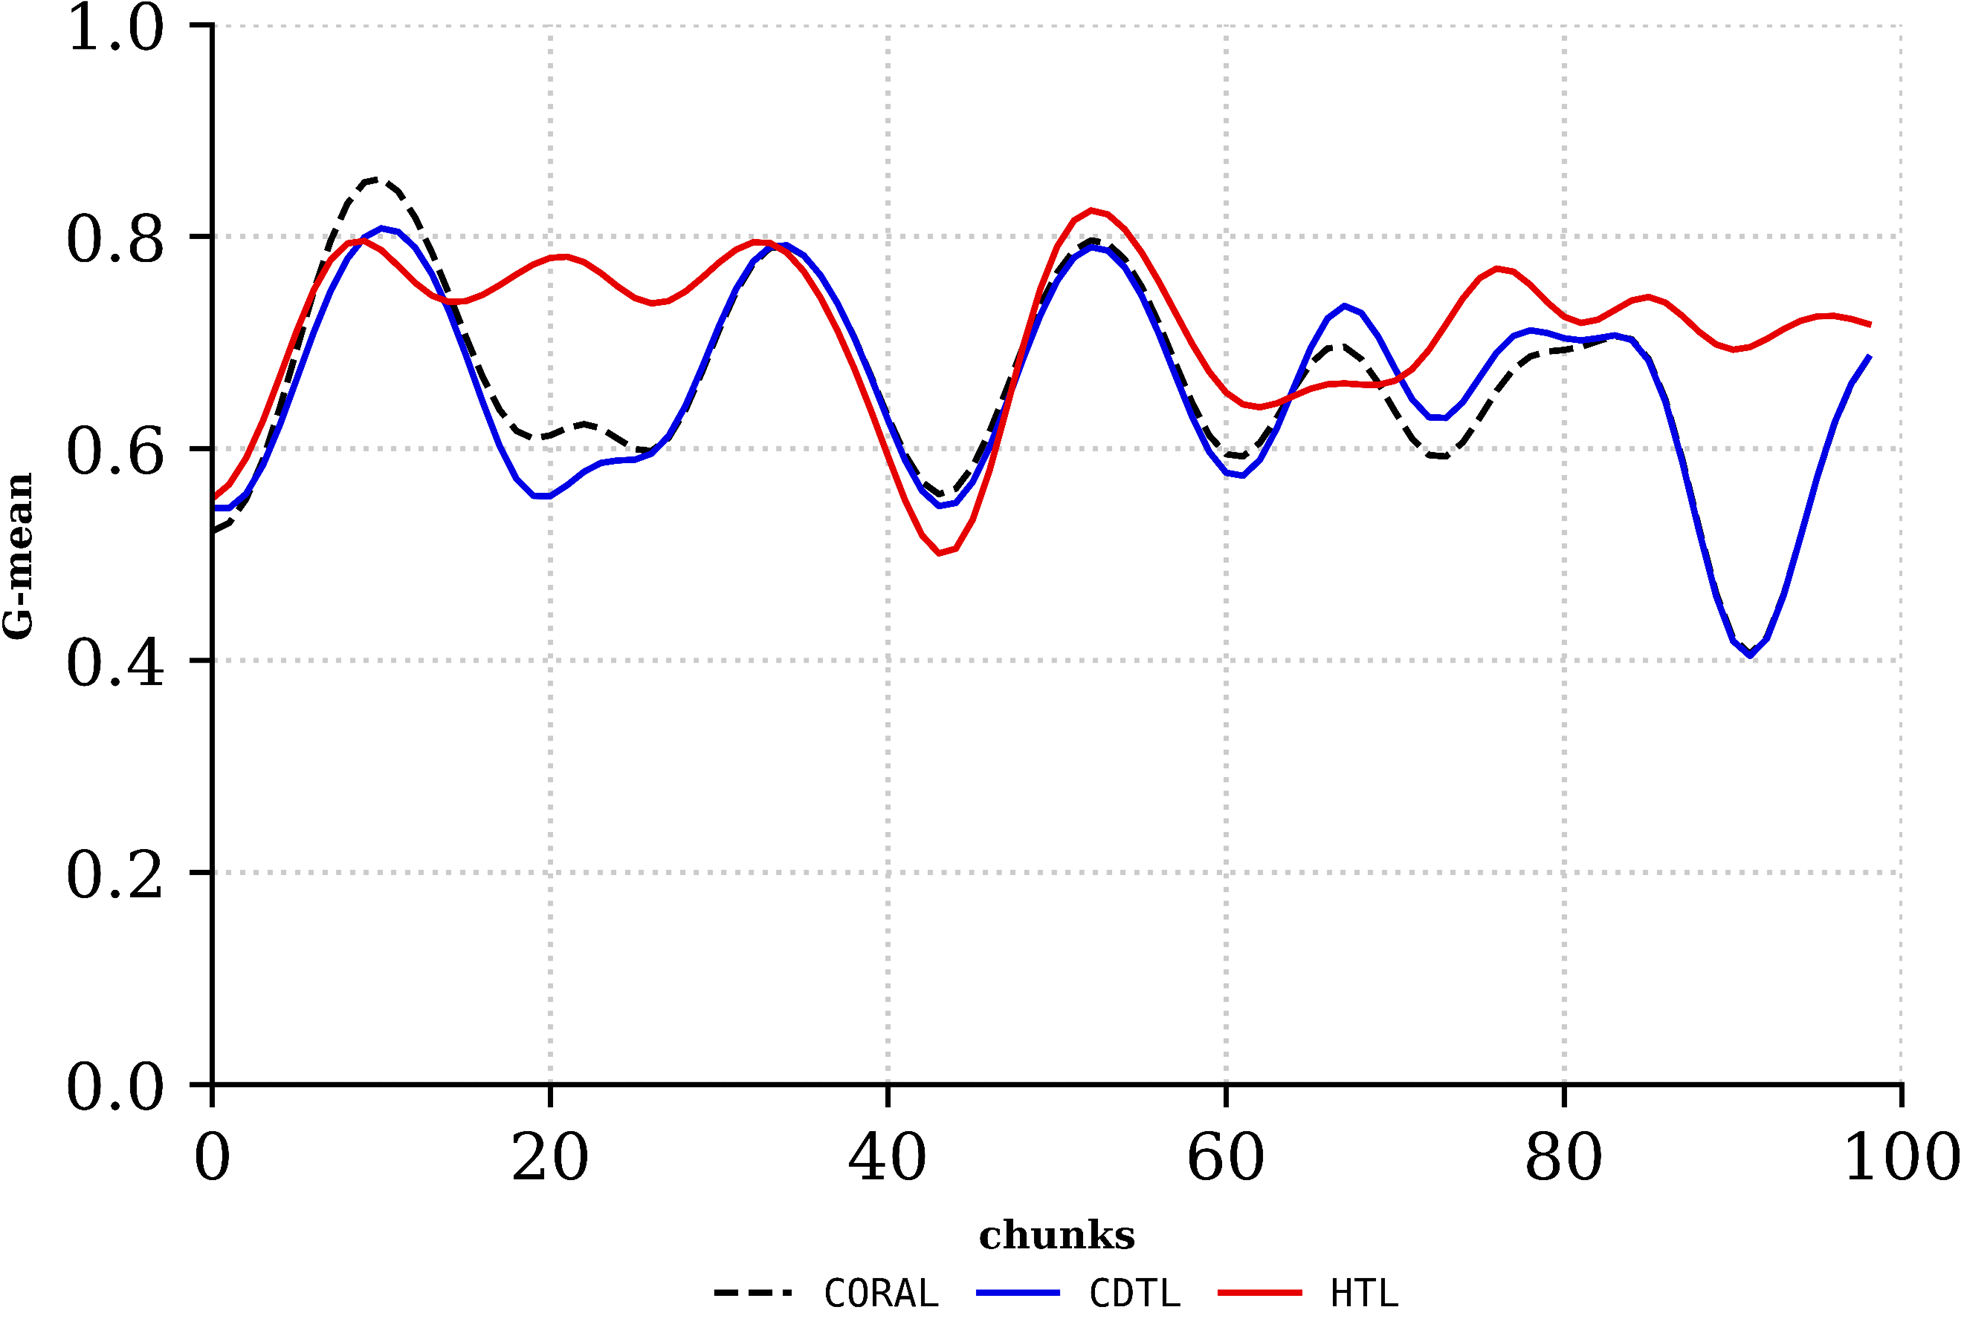
\includegraphics[width=1\linewidth]{6_transfer_learning/figures/exp1_0.png}
	\caption{Result of the Covertype Stream as the Target Domain without the Presence of the Source Domain.}
	\label{fig:6_exp1}
\end{figure}
\begin{figure}[!ht]
	\centering
	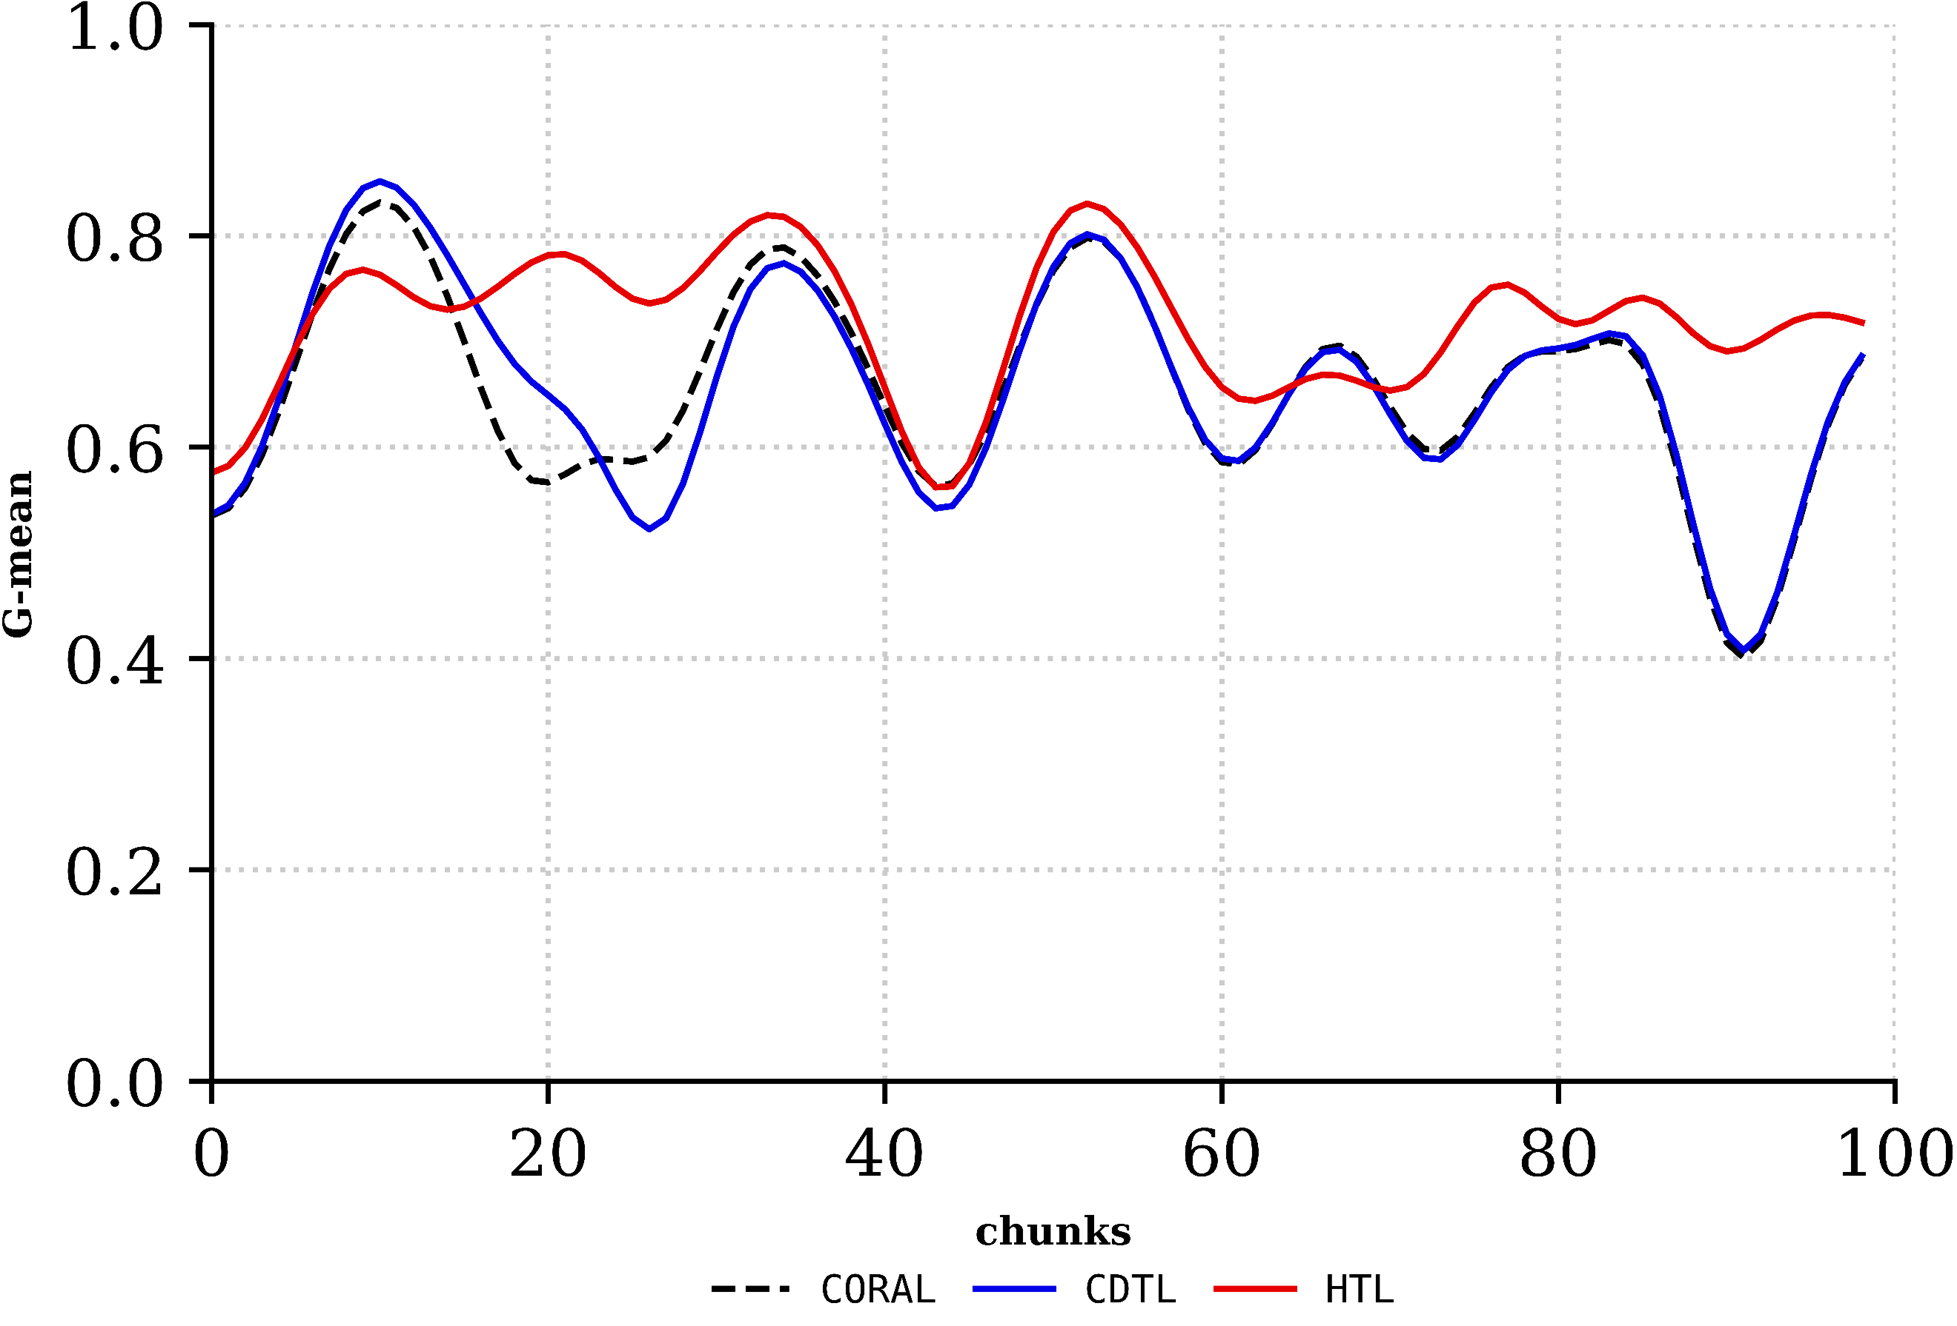
\includegraphics[width=1\linewidth]{6_transfer_learning/figures/exp1_1.png}
	\caption{Result of the Covertype Stream as the Target Domain and Homogeneous Source Domains.}
	\label{fig:6_exp2}
\end{figure}

\subsubsection{Results on the Homogeneous Source Domains Dataset}
Fig. \ref{fig:6_exp2} depicts the results of applying the compared methods to the Covertype data stream as the target domain and Synthetic-52 as a homogenous source domain, which has the same dimensionality as the Covertype stream (52 features and seven classes). Upon examining the line diagram, it becomes evident that HTL's performance in the first eight chunks may be suboptimal due to the insufficient number of classifiers available. However, following the initial eight chunks, the addition of more classifiers results in an improvement in HTL's performance. In contrast, CDTL maintains satisfactory performance throughout the chunks, while MLSMOTE consistently displays lower performance. It is important to note that HTL consistently achieves the highest performance across all chunks in the diagram. Notably, the CDTL and HTL methods in Fig. \ref{fig:6_exp2} demonstrated superiority over the same methods in Fig. \ref{fig:6_exp1}. This is attributed to the experiment shown in Fig. \ref{fig:6_exp2}, which incorporates Synthetic-52 as a source domain, thereby enhancing the performance of the methods. In contrast to the experiment in Fig. \ref{fig:6_exp1}, which lacks a source domain.

\begin{figure}[!ht]
	\centering
	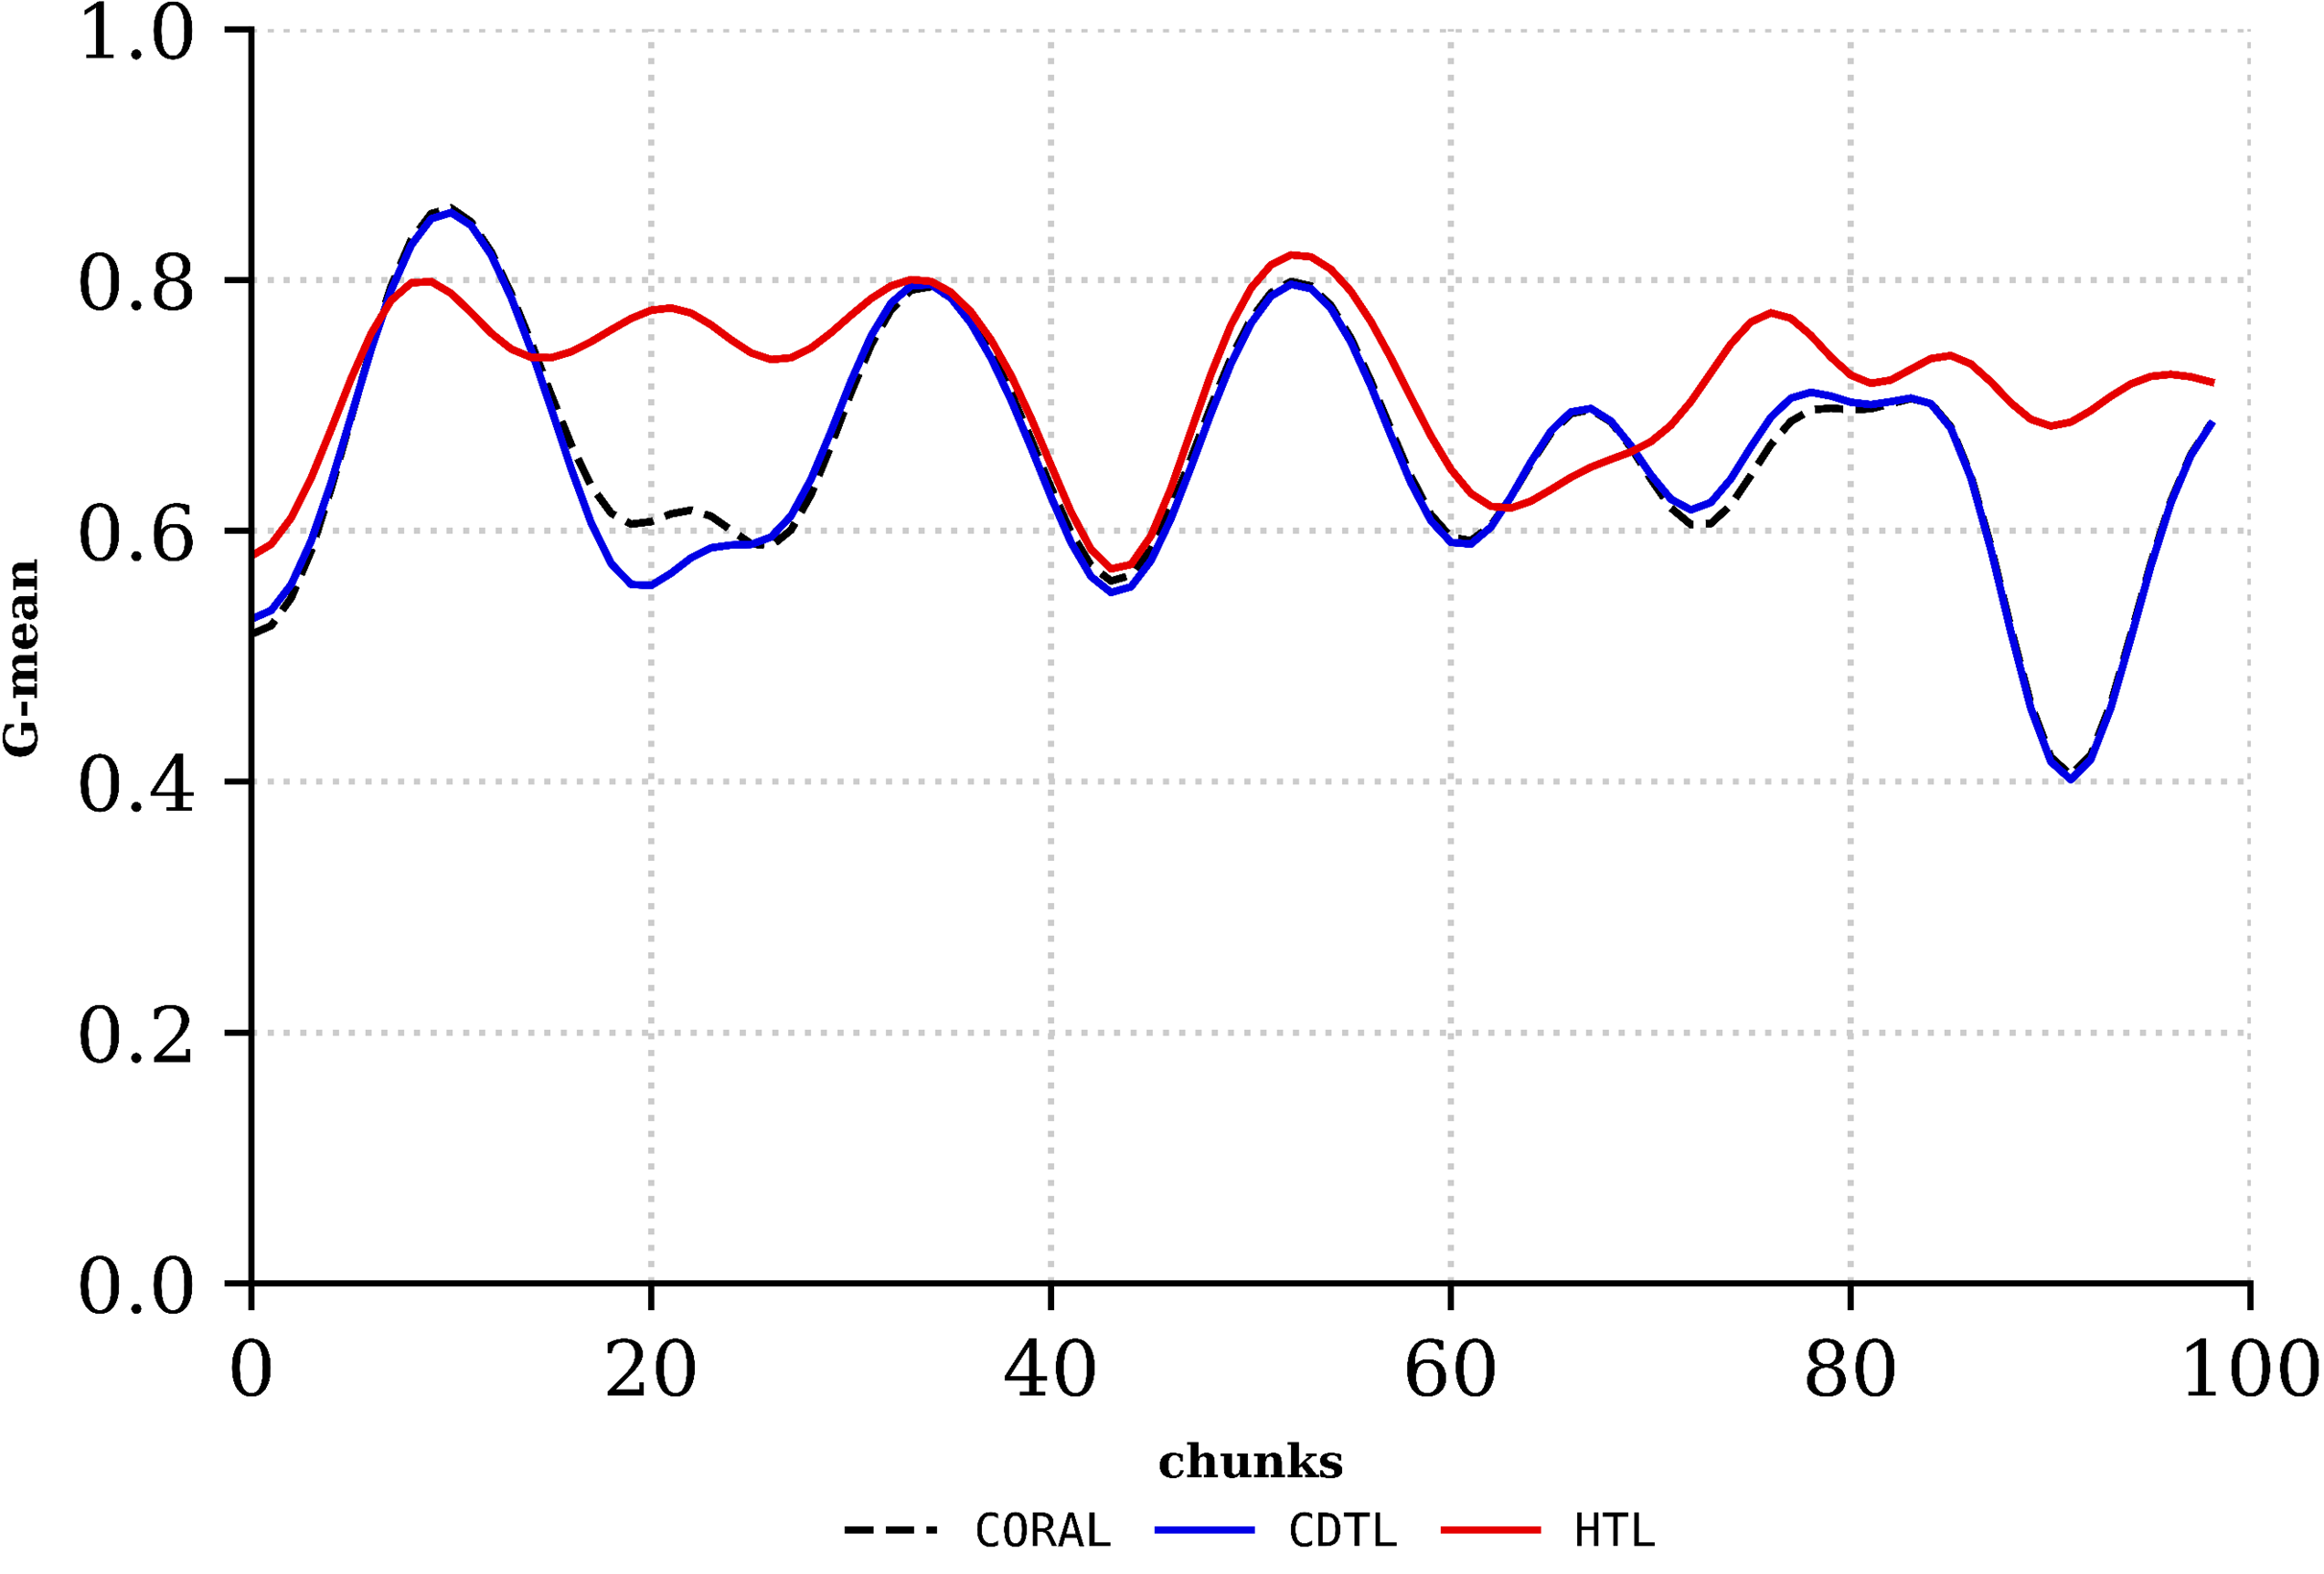
\includegraphics[width=1\linewidth]{6_transfer_learning/figures/exp2_0.png}
	\caption{Result of the Covertype Stream as the Target Domain and One Heterogeneous Source Domain.}
	\label{fig:6_exp3}
\end{figure}
\begin{figure}[!ht]
	\centering
	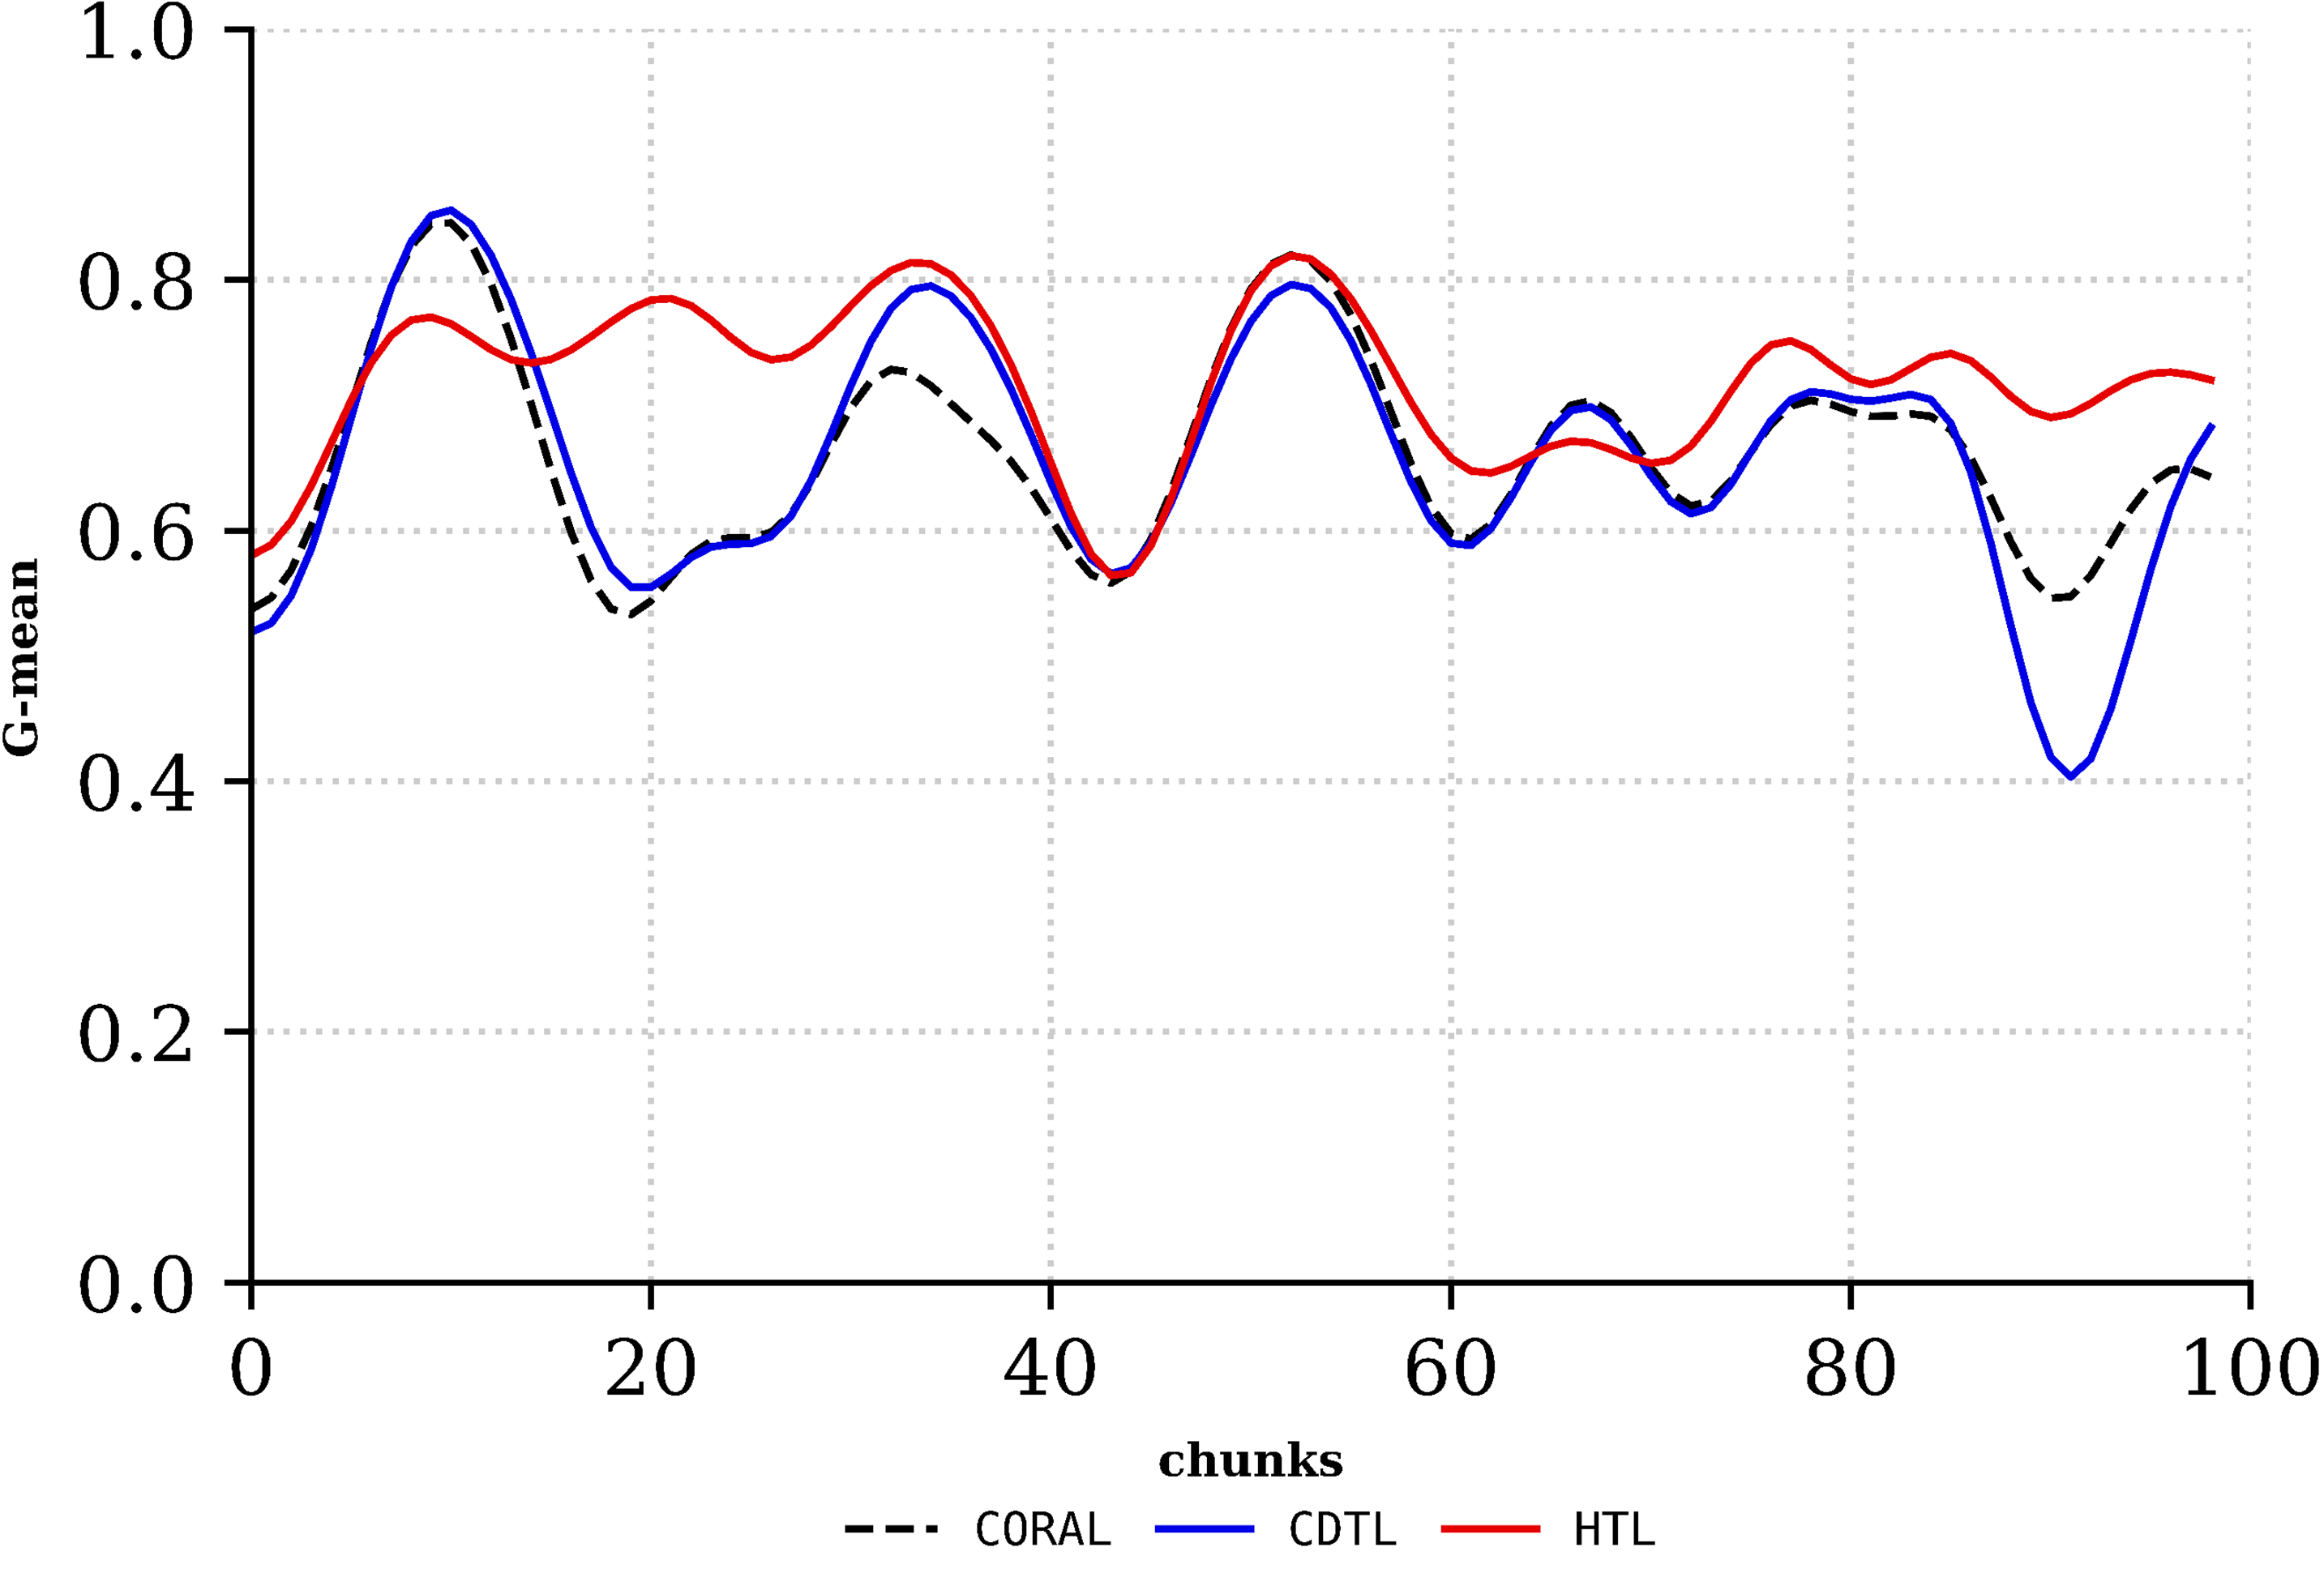
\includegraphics[width=1\linewidth]{6_transfer_learning/figures/exp2_1.png}
	\caption{Result of the Covertype Stream as the Target Domain and Multiple Heterogeneous Source Domains.}
	\label{fig:6_exp4}
\end{figure}
\begin{figure}[!ht]
	\centering
	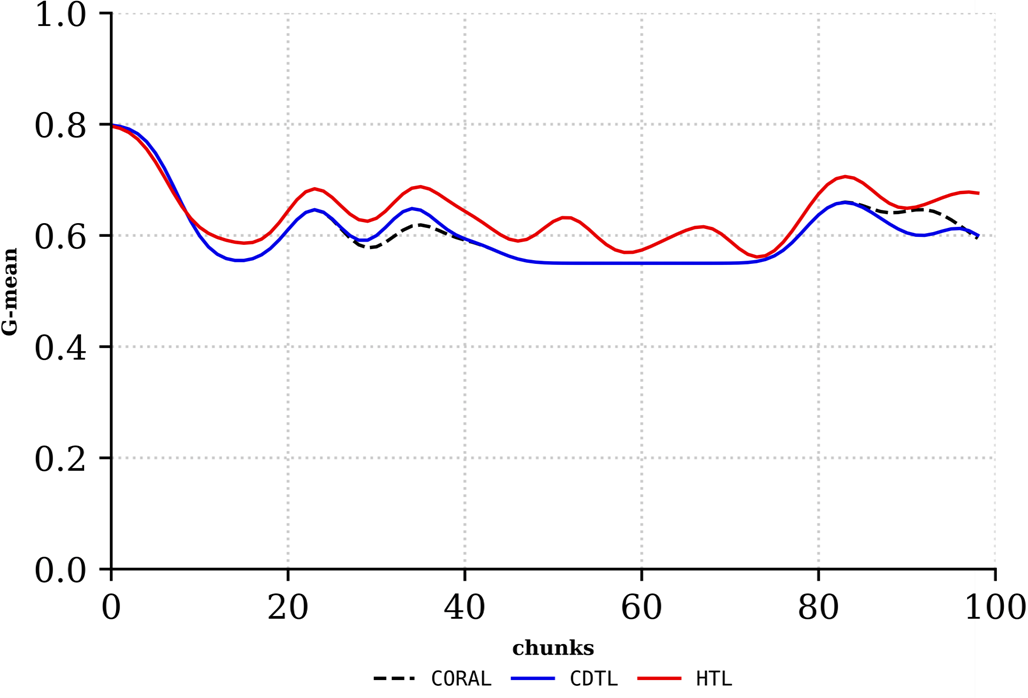
\includegraphics[width=1\linewidth]{6_transfer_learning/figures/exp3.png}
	\caption{Result of the Sensor Stream as the Target Domain and Multiple Heterogeneous Source Domains.}
	\label{fig:6_exp5}
\end{figure}

\subsubsection{Results on One Heterogeneous Source Domain}
In this experiment, the Synthetic-8 stream was utilized as a heterogeneous source domain. Considering the nature of the HTL algorithm, which can operate with heterogeneous sources, specific adjustments were implemented to enable CORAL and CDTL, which typically do not operate with such sources, to function in a heterogeneous domain environment. The eigenvector technique was applied to CORAL and CDTL to facilitate compatibility with the heterogeneous sources. Fig. \ref{fig:6_exp3} shows the results of applying the compared methods to the Covertype data stream as the target domain, with Synthetic-8 acting as the heterogeneous source domain. Synthetic-8 has a different dimensionality (eight features and four classes) compared with the Covertype stream. An analysis of the line diagram reveals that the performance of the compared approaches may vary across different chunks depending on the source domain and the positive knowledge it contributes. HTL consistently outperforms, achieving the highest performance across almost all chunks, whereas CDTL and CORAL show lower performance.

\begin{figure}[!ht]
	\centering
	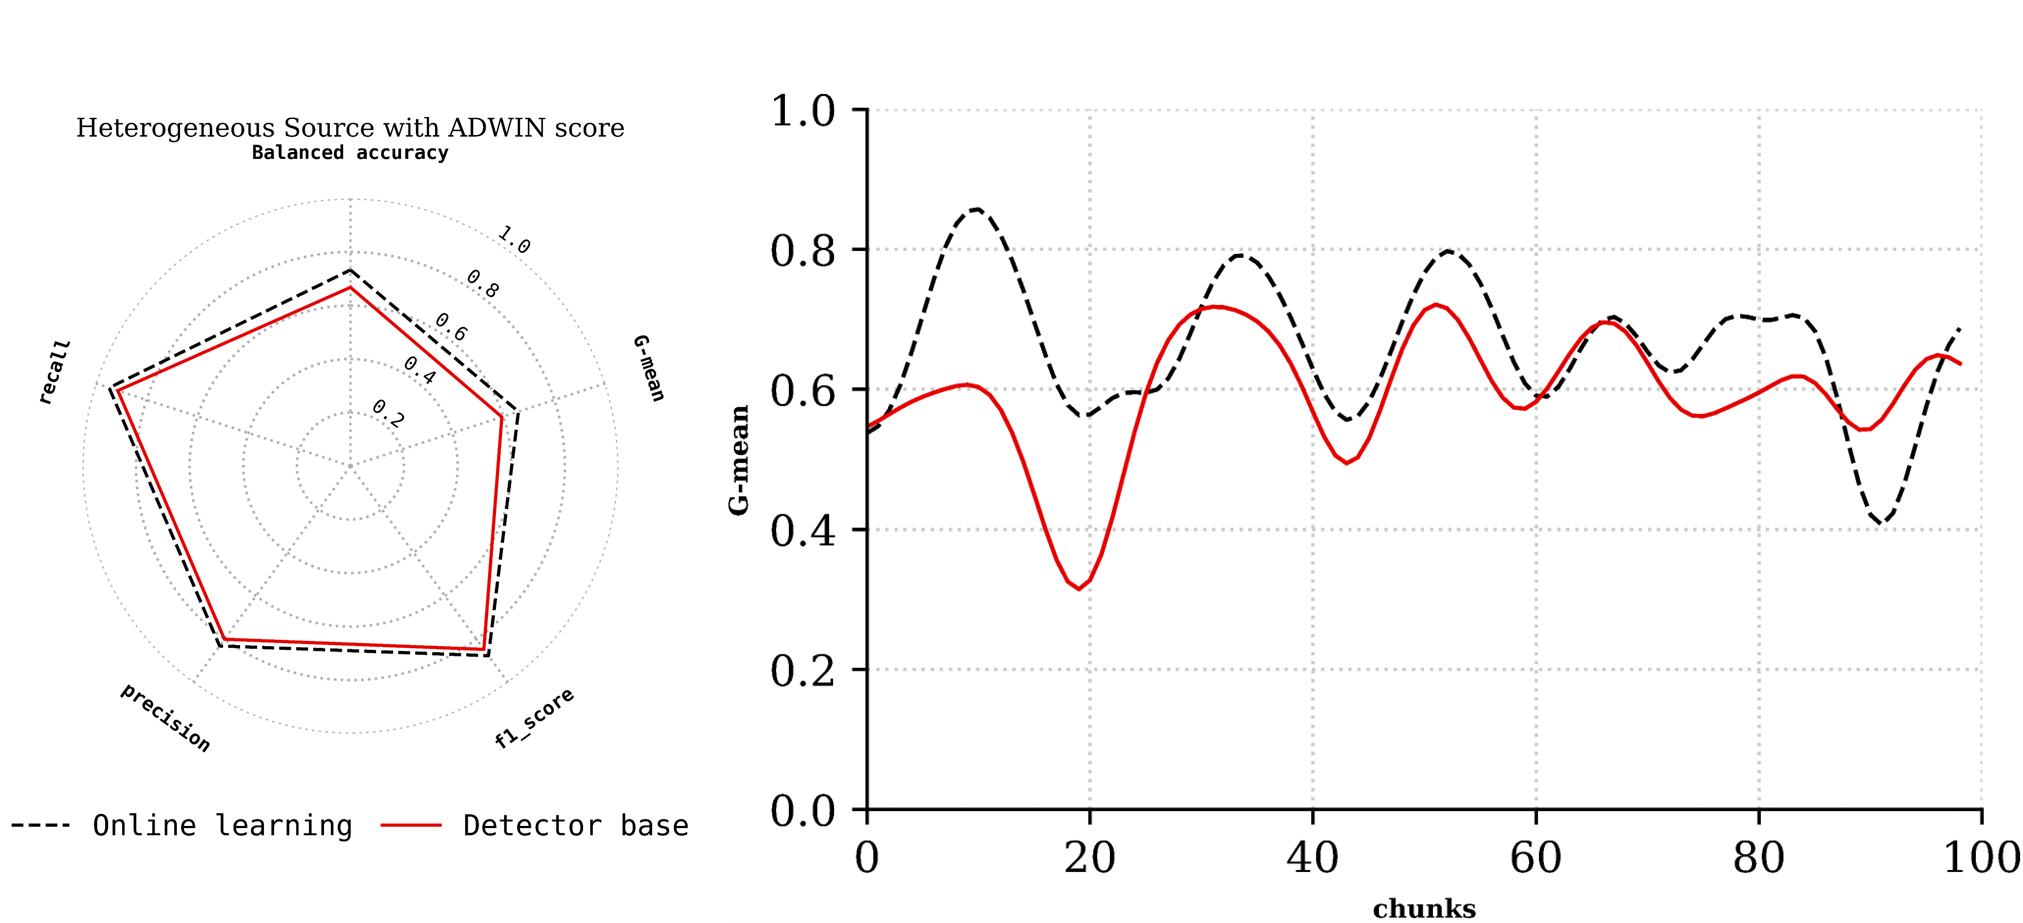
\includegraphics[width=1\linewidth]{6_transfer_learning/figures/exp4.png}
	\caption{Online learning and detector chunk-based result in Covertype stream via ADWIN detector}
	\label{fig:6_exp6}
\end{figure}

\begin{figure}[!ht]
	\centering
	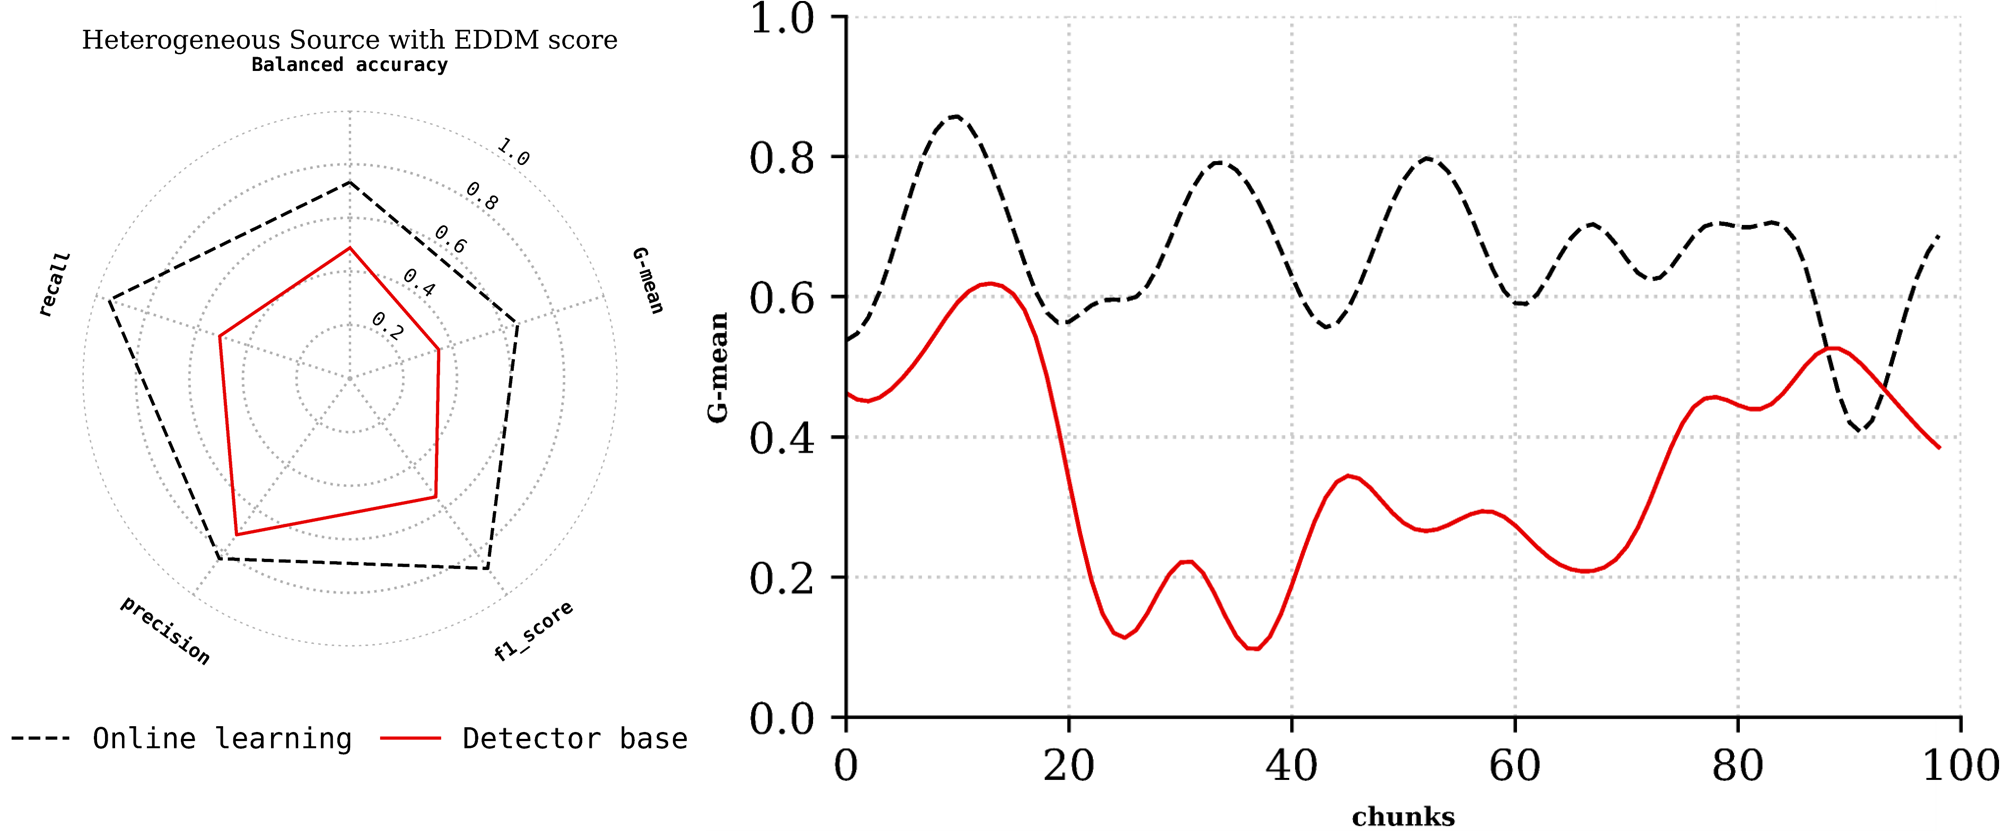
\includegraphics[width=1\linewidth]{6_transfer_learning/figures/exp5.png}
	\caption{Online learning and detector chunk-based result in Covertype stream via DDM detector}
	\label{fig:6_exp7}
\end{figure}


\subsubsection{Results on All Heterogeneous Source Domains Stream and Covertype Stream as the Target Domain}
Fig. \ref{fig:6_exp5} presents the results of applying the compared methods to the Covertype data stream as the target domain, with the Synthetic-8, Synthetic-52, and Sensor streams serving as heterogeneous source domains. From the analysis, the performance in this figure exceeds that in Fig. \ref{fig:6_exp5}. This improvement is likely due to the larger number of source domains in this experiment, which leads to an incremental increase in positive knowledge with each added source domain, consequently improving method performance. In Fig. \ref{fig:6_exp6}, the same experimental setup was employed, but the target domain was switched from the cover type to the sensor stream. Additionally, the Covertype stream was included as one of the source domains in this configuration. This modification was intended to evaluate the performance of the HTL across the various target streams. Fig. \ref{fig:6_exp6} shows that the performance of all methods might be lower than that of the Covertype stream, mainly because of the increased noise in the sensor stream and numerous drifts. However, HTL consistently outperforms, achieving the highest performance across all chunks, whereas CORAL and CDTL display nearly identical values in most chunks.

\subsubsection{Results on One Heterogeneous Source Domain}
This section presents the overall performances of the compared methods (CORAL, CDTL, and HTL) across five key performance metrics: F1 score, precision, recall, G-mean, and BAG. Table 2 showcases the performance of each method across different experiments for the five metrics. The table illustrates the average value of each metric, which represents the overall performance of each method for 100 chunks. The emphasis on the bold highlighting in the table underscores the superiority of the HTL algorithm in various source domain configurations. In the first experiment (without the source domain), CORAL showed the best performance in terms of precision, while HTL demonstrated the best performance in the other metrics. Furthermore, in most experiments, HTL outperformed the other methods across most metrics, except for the recall metric in the third experiment, in which CDTL achieved the best performance. Notably, each subsequent experiment demonstrated improved performance compared with the previous experiment. This trend arose from the incremental nature of the source domain in each experiment. The incremental addition of the source domain enhances the positive knowledge of each experiment, leading to an increased performance of the compared methods in most experiments.

\begin{table}[h]
  \centering
  \caption{The Comprehensive Performance of CORAL, CDTL, and HTL Across All Previous Experiments}
  \label{table:6_table2}
  \begin{tabular}{|l|l|c|c|c|}
  \hline
  \textbf{Experiment}                            & \textbf{Metric} & \textbf{CORAL} & \textbf{CDTL} & \textbf{HTL} \\ \hline
  \multirow{4}{*}{Without source domain}         & BAC             & 0.723          & 0.723         & \textbf{0.725} \\ \cline{2-5} 
                                                 & G-mean          & 0.652          & 0.654         & \textbf{0.717} \\ \cline{2-5} 
                                                 & F1-score        & 0.875          & 0.874         & \textbf{0.890} \\ \cline{2-5} 
                                                 & Precision       & 0.827          & 0.823         & \textbf{0.851} \\ \cline{2-5} 
                                                 & Recall          & \textbf{0.950} & 0.944         & 0.939          \\ \hline
  \multirow{4}{*}{Homogenous source domain}      & BAC             & 0.731          & 0.730         & \textbf{0.755} \\ \cline{2-5} 
                                                 & G-mean          & 0.658          & 0.653         & \textbf{0.717} \\ \cline{2-5} 
                                                 & F1-score        & 0.876          & 0.875         & \textbf{0.858} \\ \cline{2-5} 
                                                 & Precision       & 0.830          & 0.829         & \textbf{0.851} \\ \cline{2-5} 
                                                 & Recall          & 0.950          & 0.950         & \textbf{0.953} \\ \hline
  \multirow{4}{*}{Single heterogeneous source domain} & BAC         & 0.732          & 0.732         & \textbf{0.757} \\ \cline{2-5} 
                                                 & G-mean          & 0.661          & 0.657         & \textbf{0.717} \\ \cline{2-5} 
                                                 & F1-score        & 0.875          & 0.875         & \textbf{0.859} \\ \cline{2-5} 
                                                 & Precision       & 0.835          & 0.835         & \textbf{0.851} \\ \cline{2-5} 
                                                 & Recall          & 0.947          & 0.950         & \textbf{0.953} \\ \hline
  \multirow{4}{*}{Multi-source heterogeneous domain (Covertype stream)} & BAC & 0.732  & 0.732         & \textbf{0.757} \\ \cline{2-5} 
                                                 & G-mean          & 0.661          & 0.661         & \textbf{0.717} \\ \cline{2-5} 
                                                 & F1-score        & 0.875          & 0.875         & \textbf{0.859} \\ \cline{2-5} 
                                                 & Precision       & 0.835          & 0.835         & \textbf{0.851} \\ \cline{2-5} 
                                                 & Recall          & 0.947          & 0.950         & \textbf{0.953} \\ \hline
  \multirow{4}{*}{Multi-source heterogeneous domain (Sensor stream)} & BAC & 0.998  & 0.998         & \textbf{0.998} \\ \cline{2-5} 
                                                 & G-mean          & 0.971          & 0.971         & \textbf{0.992} \\ \cline{2-5} 
                                                 & F1-score        & 0.997          & 0.997         & \textbf{0.997} \\ \cline{2-5} 
                                                 & Precision       & 0.998          & 0.998         & \textbf{0.998} \\ \cline{2-5} 
                                                 & Recall          & 0.998          & 0.998         & \textbf{0.998} \\ \hline
  \end{tabular}
  \end{table}

\subsection{4.3.	Analysis Runtime between CORAL, CDTL, and HTL Techniques}
Our experimental results highlight that the selection of the optimal algorithm for handling heterogeneous transfer learning is influenced by various factors. These factors include the dataset characteristics and runtime requirements of the algorithm. In the experiments, the focus was on analyzing the runtimes of different algorithms, and the results were insightful. Notably, the HTL algorithm was exceptionally efficient. For example, when considering the training of the first experience (homogeneous source domain), the HTL algorithm completed 100 iterations within 304 seconds. In contrast, the CORAL and CDTL algorithms require more time to achieve the same number of training iterations. Furthermore, the HTL algorithm consistently demonstrated remarkable efficiency, particularly when the source domain settings were absent, single heterogeneous, or multisource heterogeneous. These findings highlight the superior runtime performance of the HTL algorithm, positioning it as an attractive choice for scenarios with stringent time constraints. The bold highlighting in Table 3 further accentuates the efficiency of the HTL algorithm across various source domain settings, including homogeneous, absent, single heterogeneous, and multi-source heterogeneous settings, making it a compelling option for applications where time efficiency is of paramount importance.

\begin{table}[h]
  \centering
  \caption{Runtimes (in seconds) for CORAL, CDTL, and HTL}
  \label{table:6_table3}
  \begin{tabular}{|l|l|l|c|c|c|}
  \hline
  \textbf{Experience}                              & \textbf{Target domain} & \textbf{Source Domain}                      & \textbf{CORAL} & \textbf{CDTL} & \textbf{HTL} \\ \hline
  without source domain                            & Covertype              & None                                         & 312            & 312           & \textbf{304} \\ \hline
  Homogenous source domain                         & Covertype              & Synthetic-52                                 & 6165           & 614           & \textbf{606} \\ \hline
  Single heterogeneous source domain               & Covertype              & Synthetic-8                                  & 6060           & 4703          & \textbf{4475} \\ \hline
  Multi-source heterogeneous domain                & Covertype              & Sensor, Synthetic-52, and Synthetic-8        & 23011          & 14043         & \textbf{13824} \\ \hline
  Multi-source heterogeneous domain                & Sensor                 & Covertype, Synthetic-52, and Synthetic-8     & 14524          & 3052          & \textbf{3005} \\ \hline
  \end{tabular}
  \end{table}
  
\subsection{4.4.	Analysis accuracy and runtime of HTL for online learning and chunk-based concept drift}
We conducted a thorough series of statistical analyses encompassing 12 comparisons across three diverse datasets, three methods, and two drift detectors. These analyses were rigorously evaluated using a non-parametric test, specifically the Kruskal-Wallis test. The results of this test were striking, revealing substantial variations in the G-mean measurements across most experiments. Importantly, these differences were not due to random chance \cite{yamada2013change}. Upon closer examination of the assessments for the three methods, PA, MLSMOTE, and MLSOTE, as detailed in Table \ref{tab:4_first_proposal_result_table_3}, we found compelling evidence supporting the acceptance of the null hypothesis (H0).
This implies that the expected and observed data exhibited statistically significant disparities. H0 is rejected when significant differences are not observed and H0 is accepted if the P-value falls below the critical value. Underlining the significance of our analysis, the Kruskal-Wallis test was conducted with a 95\% confidence level, and the P-value was rounded to the first three digits after the decimal point. Nevertheless, it is important to note that a similarity in the performances of the methods emerged in the third and fourth experiments, resulting in the rejection of H0. This similarity can be attributed to the fact that the DDM detected fewer drifts in these experiments.

\begin{table}[h]
  \centering
  \caption{Runtimes (in seconds) for Online Learning, ADWIN, and EDMM drift detector}
  \label{table:6_table4}
  \begin{tabular}{|l|c|c|}
  \hline
  \textbf{Technique}       & \textbf{Runtime} & \textbf{Learning Times} \\ \hline
  Online Learning          & 3102             & 100                     \\ \hline
  ADWIN detector           & 2257             & 63                      \\ \hline
  EDMM detector            & 1948             & 40                      \\ \hline
  \end{tabular}
  \end{table}
  